\section{Gaussian Process Fundamentals}\label{sec:gp_fundamentals}

This section reviews the basics of \gls[hyper=false]{gp}.
The connection between the stochastic process and multivariate Gaussian random variable (Gaussian random vector) is first established.
Appendix~\ref{app:probability} gives some the basic concepts of multivariate random variable such as joint, marginal, and conditional probabilities.

\subsection[Multivariate Normal Random Variable]{Multivariate Gaussian (Normal) Random Variable}\label{sub:gp_mvn}

Multivariate Normal (or Gaussian and hereinafter, \textsc{MVN}) random variable is the most widely studied and applied random variable.
There are several reasons for this.
From a practical viewpoint, 
the distribution of MVN is tractable and 
its special properties are well known (citation needed).
From an epistemological point of view, as MVN distribution is fully characterized by its mean and covariance, only these wo parameters are of interest.
Furthermore, any dependence withing structure within a set of data can sufficiently be described linearly through the notion of statistical covariance.

This section reviews the definition and some of the most important properties of MVN random variable relevant in the present study.
In the next section, the MVN random variable is generalized to be defined on infinite-dimensional space through the notion of Gaussian stochastic process.

A collection of $D$ random variables $\mathbf{X} = [X_1, X_2, ...,X_D] \in \mathbb{R}^D$ is said to have a multivariate normal distribution with mean vector $\boldsymbol{\mu} \in \mathbb{R}^D$ and variance-covariance matrix $\boldsymbol{\Sigma} \in S_{++}^D$ if its joint probability density function is given by,

\begin{equation}
p(\mathbf{x};\boldsymbol{\mu},\boldsymbol{\Sigma}) = \frac{1}{2\pi^{D/2}|\boldsymbol{\Sigma}|^{1/2}} \exp{\left[-\frac{1}{2}(\boldsymbol{x}-\boldsymbol{\mu})^T\boldsymbol{\Sigma}^{-1}(\boldsymbol{x}-\boldsymbol{\mu})\right]}
	\label{eq:gaussian_joint_density}
\end{equation}

The joint distribution of MVN random variable is parameterized and fully specified by the mean vector $\boldsymbol{\mu}$ and the variance-covariance matrix $\boldsymbol{\Sigma}$. The symbol ``;'' separates the value of the variates $\boldsymbol{x}$ from the parameters of the distribution. 
A $D$-variate random variable $\boldsymbol{X}$ distributed as multivariate normal is written as,

\begin{equation}
	\boldsymbol{X} \sim \mathcal{N}_D\left(\boldsymbol{\mu}, \boldsymbol{\Sigma}\right)
\end{equation}

where $\mathbb{E}$ is the expectation operator.

The variance-covariance matrix $\boldsymbol{\Sigma}$ is an element in the space of symmetric positive definite (PSD) $D \times D, S_{++}^D$ defined as,

\begin{equation}
	S_{++}^D = \{A \in \mathbb{R}^{D\times D}: A = A^T and \mathbf{x}^T A \mathbf{x} \geq 0, \forall \mathbf{x} \in \mathbb{R}^D \textnormal{and } \mathbf{x} \neq 0 \}
	\label{eq:def_covariance_matrix}
\end{equation}

% Why Gaussian

% Definition of Gaussian Random Vector

% Joint Distribution

% Mean Vector

% Variance-Covariance Matrix

% Diagonal Elements of the Variance-Covariance Matrix
The diagonal elements of the variance-covariance matrix, $\Sigma_{i,i}$, describe the variance of a single random variable,
while the off-diagonal elements, $\Sigma_{i,j}$, describe the covariation between a pair of random variables,
\begin{equation}
	\boldsymbol{\Sigma} =
	\begin{pmatrix}
			\mathbf{V}[\mathbf{Z}_1] & \cdots                & \text{Cov}[\mathbf{Z}_1, \mathbf{Z}_L] \\
			\vdots                   & \ddots                & \vdots \\
			\text{Cov}[\mathbf{Z}_L, \mathbf{Z}_1] & \ddots & \mathbf{V}[\mathbf{Z}_L]
	\end{pmatrix}
\label{eq:covariance_matrix}
\end{equation}
where $\mathbb{V} [\circ]$ and $\text{Cov} [\circ]$ are the variance and covariance operators, respectively. 

% Partitioning Gaussian Random Vector
Suppose that $\mathbf{Z}$ is partitioned into two sub-vectors (two disjoint sets) $\mathbf{Z}_A$ and $\mathbf{Z}_B$ such that $\mathbf{Z} = [\mathbf{Z}_A, \mathbf{Z}_B]$ 
(see Appendix~\ref{app:probability}).
Then the Gaussian random vector $\mathbf{Z} = [\mathbf{Z}_A, \mathbf{Z}_B]$ can be written as,
\begin{equation}
	\begin{pmatrix}
		 \mathbf{Z}_A \\
		 \mathbf{Z}_B
	\end{pmatrix} \sim \mathcal{N} \left (
	\begin{pmatrix}
			\boldsymbol{\mu_A} \\
			\boldsymbol{\mu_B}
	\end{pmatrix}, \begin{pmatrix}
		  \boldsymbol{\Sigma_{1,1}}   & \boldsymbol{\Sigma_{1,2}} \\
			\boldsymbol{\Sigma^T_{1,2}} & \boldsymbol{\Sigma_{2,2}} \\
	\end{pmatrix} \right)
\label{eq:gaussian_random_vector}
\end{equation}

with $\mathbf{Z}_A \in \mathcal{Z} \subseteq \mathbb{R}^{D_1}$, $\mathbf{Z}_A \in \mathcal{Z} \subseteq \mathbb{R}^{D_2}$, and $D = D_1 + D_2$ 

% Marginal Distribution of Gaussian Random Vector
The marginal density of both $\mathbf{Z}_A$ and $\mathbf{Z}_B$ also follows a multivariate Gaussian distribution given as,
\begin{equation}
	\begin{split}
		p(\mathbf{z}_A) & = \frac{1}{2\pi^{D/2}|\boldsymbol{\Sigma_{1,1}}|^{1/2}} \exp{\left[-\frac{1}{2}(\mathbf{z}_A-\boldsymbol{\mu}_A)^T\boldsymbol{\Sigma^{-1}_{1,1}}(\mathbf{z}_A-\boldsymbol{\mu}_B)\right]} \\
		p(\mathbf{z}_B) & = \frac{1}{2\pi^{D/2}|\boldsymbol{\Sigma_{2,2}}|^{1/2}} \exp{\left[-\frac{1}{2}(\mathbf{z}_B-\boldsymbol{\mu}_B)^T\boldsymbol{\Sigma^{-1}_{2,2}}(\mathbf{z}_A-\boldsymbol{\mu}_B)\right]}
	\end{split}
\label{eq:gaussian_marginal}
\end{equation}

% Conditional Distribution of Gaussian Random Vector
Similarly, the conditional density of $\mathbf{Z}_A$ conditioned on $\mathbf{Z}_B$ also follows a multivariate Gaussian distribution given as,
\begin{equation}
	\begin{split}
		& p(\mathbf{z}_A|\mathbf{z}_B) = \frac{1}{2\pi^{D/2}|\boldsymbol{\Sigma_{1,1}}|^{1/2}} \exp{\left[-\frac{1}{2}(\mathbf{z}_A-\boldsymbol{\mu}_A)^T\boldsymbol{\Sigma^{-1}_{1,1}}(\mathbf{z}_A-\boldsymbol{\mu}_B)\right]} \\
		& \boldsymbol{\mu}_A = \boldsymbol{\mu}_A + \boldsymbol{\Sigma}_{1,2} \boldsymbol{\Sigma}^{-1}_{2,2} \left(\mathbf{z}_B - \boldsymbol{\mu}_B \right) \\
		& \boldsymbol{\Sigma}^*_{1,1} = \boldsymbol{\Sigma}^*_{1,1} - \boldsymbol{\Sigma}_{1,2} \boldsymbol{\Sigma}^{-1}_{2,2} \boldsymbol{\Sigma}^T_{1,2} 
	\end{split}
\label{eq:gaussian_conditional}
\end{equation}
The results are analagous for $p(\mathbf{z}_B|\mathbf{z}_A)$. 
The proofs of these special properties of the MVN are provided in Appendix~\ref{app:gaussian_identities}.

% Illustration of Joint, Marginal, and Conditional
To illustrate the notions of joint, marginal, and conditional distributions, an example of a bivariate random variable, a random vector $Z = [Z_1, Z_2] \in \mathbb{R}^2$ is given.
\marginpar{random vector, an example}
It has the following mean vector and variance-covariance matrix, respectively,
\begin{equation}
	\begin{split}
		\begin{pmatrix}
			Z_1 \\
			Z_2
		\end{pmatrix} & \sim \mathcal{N}(\boldsymbol{\mu}, \boldsymbol{\Sigma}) \\
		 \boldsymbol{\mu} & = [0, 0]^T \\
		  \boldsymbol{\Sigma} = 
				\begin{pmatrix}
					\mathbf{V}[\mathbf{Z}_1]                & \text{Cov}[\mathbf{Z}_1, \mathbf{Z}_2]\\
					\text{Cov}[\mathbf{Z}_2, \mathbf{Z}_1]  & \mathbf{V}[\mathbf{Z}_2]\\
			\end{pmatrix} & =
			\begin{pmatrix}
					0.5       & -0.265165\\
					-0.265165 & 0.25\\
			\end{pmatrix}
	\end{split}
\label{eq:ex_bivariate}
\end{equation}
The joint, marginal, and conditional probability distributions of random vector $\mathbf{Z}$ are illustrated in Fig.~\ref{fig:plot_bivariate_normal}.
\begin{figure}[bth]
	\centering
	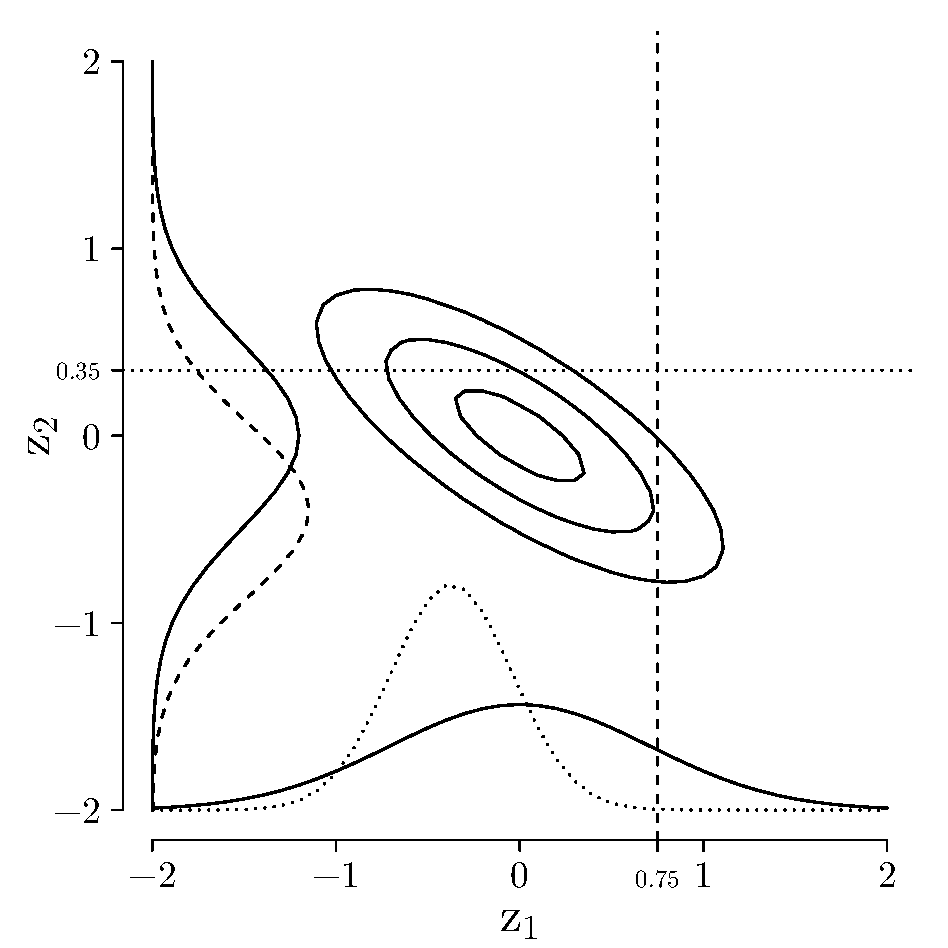
\includegraphics[scale=0.50]{../figures/chapter4/figures/plotBivariateNormal.pdf}
	\caption[Illustration of a bivariate Gaussian distribution]{An illustration of bivariate Gaussian distribution of random vector $Z = [Z_1, Z_2]$ having marginal means of $0.0$ and variances of $0.5$ and $0.25$, respectively and with covariance of $-0.265165$. The solid ellipsoids indicate the contour of joint density of random vector $[Z_1, Z_2]$. The two solid curves at the $x$- and $y$-axes indicate the marginal densities of $Z_1$ and $Z_2$, respectively. The dotted curve shows the conditional density of random variable $Z_1$ given $z_2 = 0.35$, while the dashed curve shows the conditional density of $Z_2$ given $z_1 = 0.75$.}
	\label{fig:plot_bivariate_normal}
\end{figure}

The joint density for Gaussian random vector is given in Eq.~(\ref{eq:gaussian_joint_density}.
\marginpar{joint density, illustrated}
For the bivariate random variable in the example, the density can be shown as contour plot in Fig.~\ref{fig:plot_bivariate_normal}.
In the figure, the solid ellipsoids are the iso-contours of the distribution, where each pair of values lies along the contour line has the same probability density value.

The two marginal densities for the example are shown as the solid curves plotted in the $x$ and $y$-axes, respectively.
\marginpar{marginal density, illustrated}
As illustrated, the marginalization of the joint distribution can be thought as a \emph{projection} of the $2$-dimensional distribution into each of the corresponding dimension.

Finally, two conditional distributions $p(z_1|z_2=0.35)$ and $p(z_2|z_1=0.75)$ are given as examples of conditioning a probability distribution in Fig.~\ref{fig:plot_bivariate_normal}.
\marginpar{conditional density, illustrated}
They are shown as dotted and dashed curves plotted in both axes.
Instead of projection to either of the axes, conditioning can be thought of as \emph{slicing} the $2$-dimensional distribution.
Conditioning two correlated random variables on one, in general, changes the shape of the distribution of the other variable.
From the figure, conditioning shifts the mean and reduces the variance of the resulting conditional distribution. 

% Drawing from Multivariate Gaussian
There are multiple ways to draw samples from a multivariate Gaussian distribution.
One method is particular require the deco
This method, so-called \emph{Cholesky} method, is detailed in Appendix.
A random number generator for the standard univariate distribution itself is widely available in many standard numerical computing environments.
The method in Appendix is used to generate 250 samples for the bivariate.
The resulting scatter plot and sample histograms of the marginal distributions 

% From Multivariate to Infinite Variate
\gls[hyper=false]{gp} can often be thought simply as a generalization of finite multivariate Gaussian random variable into an infinite multivariate one.
\marginpar{An entry to Gaussian Process}
To illustrate this idea, the marginal and conditional distributions of the bivariate distribution depicted in Fig.~ is plotted with the random variables at the same axis ($x$) while the range pf values of the variables are plotted in another axis ($y$).
The left panels shows the marginal distributions of random variables $Z_1$ and $Z_2$, where in Fig.~ they are plotted as black curves in their respective axes.
The center panel shows an observed value of $z_1 = 0.75$ depicted in Fig.~ as vertical dashed line.
Finally the right panel shows the conditional distribution of the non-observed variable $Z_2$ given $z_1 = 0.75$, which in Fig.~ was depicted as the dashed curve in the $y$-axis.
As it can be seen, the mean and standard deviation of the conditional distribution of $Z_2$ have been shifted and reduced, respectively, according to the information about $Z_1$.

Depiction in Fig.~ can easily be extended to a larger number of random variables, provided a valid mean vector and a valid covariance matrix.
Fig.~ shows such an extension to $15$-variate Gaussian random variable.
The origin of the underlying $15 \times 15$ covariance matrix is at the moment unimportant, but what the matrix does is defining how the variables are correlated to each other.
The whole covariance matrix, except its diagonal elements, is irrelevant in describing the marginal (Fig, left),
but it is significant in describing the shape of the conditional (Fig, right) according to Eqs.~.
As before, the conditional probability of the non-observed random variables are shifted and their standard deviation are reduced due to the information provided from the observed variables.

% Closing Sentence
Gaussian stochastic generalizes this procedure beyond $2$- or $15$-variate Gaussian random variable to an arbitrary number of variables at arbitrary locations in the real line.
It is easy to imagine that the shape of both marginals and conditionals will become smoother and smoother with increasing number of random variables in the $x$-axis, thus resembling more of a smooth function.
In fact, it is one of the interpretations of Gaussian process: a distribution over functions (citation). 


\subsection{Gaussian Process}

% What is a stochastic process
Gaussian stochastic process is a particular class of \emph{stochastic} or \emph{random process}.
\marginpar{Stochastic process}
Stochastic process is a collection of random variables, each of which are often indexed with certain underlying rules or ordering.
To be precise, a stochastic process is a set of random variables $\mathbf{Y} = \{Y_i, i \in I\}$, where $I$ is an index set, 
and it is defined on a probability space $(\Omega, \mathcal{F}, \mathbb{P})$, 
where $\Omega$, $\mathcal{F}$, and $\mathbb{P}$ are the sample space, the set of events, and the assigned probability to the event, respectively \cite{Syski2014}.

% Examples of stochastic process applications
For example, a time series can be modeled using stochastic process where the random variables are the observations taken at different time ordered sequentially.
\marginpar{Stochastic process applications}
In this case the index set is the time index of the observations.
A spatial model, as another example, can be modeled as a collection of random variables indexed by their locations in space.
And finally, in the metamodeling application, the random variables are collection of computational model output values at different input values.

% Gaussian stochastic process
\emph{Gaussian stochastic process} (GP) is defined as a collection of random variables, 
\emph{arbitrary number of which is a multivariate Gaussian random variable} \cite{Rasmussen2006, Debicki2014}.
\marginpar{Gaussian process}
To establish the connection with the notion of \emph{random function}, the collection of the above random variables refers to the collection of values of a random function $Y(\circ)$ at various possible input $\mathbf{x}$ in the domain $\mathcal{X} \subseteq \mathbb{R}^D$.
Specifically, $Y(\mathbf{x}), \, \text{for} \, \mathbf{x} \in \mathcal{X} \subseteq \mathbb{R}^D$ is a \emph{Gaussian process} if and only if for any choice from the finite set of input $\{\mathbf{x}_1, \mathbf{x}_2, \cdots, \mathbf{x}_L ; \, L \geq 1\}$, the random vector $\left[Y(\mathbf{x}_1), Y(\mathbf{x}_2), \cdots, Y(\mathbf{x}_L)\right]$ is a multivariate Gaussian random variable \cite{Santner2003}.

% Basic notation
A \gls[hyper=false]{gp} is fully specified by its mean and covariance functions, instead mean vector and covariance matrix.
A \gls[hyper=false]{gp} $Y$ on $\mathcal{X} \subseteq \mathbb{R}^D$ with a given mean function $m$ and covariance $K$ is denoted as
\begin{equation}
	Y(\mathbf{x}) \sim \mathcal{GP} \left(m(\mathbf{x}), K(\mathbf{x}, \mathbf{x}^*) \right)
\label{eq:gp_notation}
\end{equation}

% Mean Function
The mean function of a Gaussian process $Y(\mathbf{x})$ is the function $m: \chi \subseteq \mathbb{R}^D \mapsto \mathbb{R}$ defined as,
\marginpar{Mean function}
\begin{equation}
	m(\mathbf{x}) = \mathbb{E}[Y(\mathbf{x})]
\label{eq:gp_mean_functions}
\end{equation}

% Covariance Function
The covariance function of a Gaussian process $Y(\mathbf{x})$, on the other hand, is the function $K: (\chi \subseteq \mathbb{R}^D) \times (\chi \subseteq \mathbb{R}^D) \mapsto \mathbb{R}$ defined as,
\marginpar{Covariance Function}
\begin{equation}
	K(\mathbf{x}_i, \mathbf{x}_j) = \text{Cov}[Y(\mathbf{x}_i), Y(\mathbf{x}_j)]
\label{eq:gp_cov_functions}
\end{equation}
Notice that while the covariance function describes the covariance describes the covariance between pair of random function values, 
it is defined only as a function of the two inputs differentiating them.
Covariance function is also sometimes referred to as the \emph{covariance kernel} function as it defines the elements of the covariance matrix (see example below).
As such, not all functions of the pair of inputs $\mathbf{x}_i, \mathbf{x}_j$ are a \emph{valid} covariance function, but only the ones that yield a valid variance-covariance matrix given by condition in Eq.~(\ref{eq:covariance_matrix}). 

% Process Variance
Finally, the process variance is defined as the covariance between two random function values at the same input,
\marginpar{Process variance}
\begin{equation}
	K(\mathbf{x}_i, \mathbf{x}_i) = \text{Cov}[Y(\mathbf{x}_i), Y(\mathbf{x}_i)] = \mathbf{V}[Y(\mathbf{x}_i)]
\label{eq:process_variance}
\end{equation}

% Gaussian Stochastic Process and Multivariate Gaussian Random Variable
For a given finite $L$, a \gls[hyper=false]{gp} is reduced to a multivariate Gaussian random variable characterized by its mean vector $\boldsymbol{\mu}$ and covariance matrix $\boldsymbol{\Sigma}$,
\begin{equation}
	\begin{split}
		& [Y(\mathbf{x}_i)] \sim \mathcal{N}(\boldsymbol{\mu}, \boldsymbol{\Sigma}) \quad ; \, i = 1, 2, \cdots, L \\
		& \boldsymbol{\mu} = [m(\mathbf{x}_1), m(\mathbf{x}_2), \cdots, (\mathbf{x}_L)]^T \\
		  & \boldsymbol{\Sigma} = 
				\begin{pmatrix}
					\mathbf{V}[Y(\mathbf{x}_1)]  & \cdots & \text{Cov}[Y(\mathbf{x}_1), Y(\mathbf{x}_L)]\\
					\vdots	& \ddots & \vdots\\
					\text{Cov}[Y(\mathbf{x}_L), Y(\mathbf{x}_1)]  & \cdots  & \mathbf{V}[Y(\mathbf{x}_L)]\\
			\end{pmatrix} \\
	\end{split}
\label{eq:gp_to_mvn}
\end{equation}

% Example, introduced
The shape of the random function drawn from a \gls[hyper=false]{gp} is characterized by its mean and covariance functions.
Brief explanations of these functions will be provided in the next two subsections.
\marginpar{fully specified GP, an example}
In the meantime, an example of a fully specified Gaussian process will be used to illustrate how samples of functions can be drawn from such a stochastic process.
For the example, the following mean and covariance function will be used
\begin{equation}
	\begin{split}
		m(\mathbf{x}) & = 0 \\
		K(\mathbf{x}, \mathbf{x}^*) & = \sigma^2 \exp{\left[-\frac{(\mathbf{x} - \mathbf{x}^*)^2}{2\theta^2}\right]} = 10 \exp{\left[-\frac{(\mathbf{x} - \mathbf{x}^*)^2}{0.98}\right]}
	\end{split}
\label{eq:gp_example}
\end{equation}
where $x$ is a $1$-dimensional input parameter such that $x \in [-2, 2]$.
The mean function is set to constant zero, while the covariance function is chosen to be the so-called \emph{Gaussian covariance function} (which will be detailed in the sequel).
The Gaussian covariance function is parameterized by the characteristic length scale $\theta$ which is set to $0.70$.
This parameter is often referred to as the \emph{hyper-parameter} of the function.
Finally, $\sigma^2$ is the common variance of the stochastic process and it is set to $10$.

% Example continued, sample path
To generate random draws of function from the fully specified \gls[hyper=false]{gp} given in Eq.~(\ref{eq:gp_example}), 
first it must be specified at which input $x$ the function values are to be drawn.
\marginpar{sample path (trajectory) of a GP}
For the present example, $x$ is chosen to be uniformly distributed $\{-2 + 0.2 \times i\}_{i=0}^{20}$.
By specifying these locations, the $21$-variates Gaussian random variable can be constructed using Eq.~(\ref{eq:gp_to_mvn}) with the elements of variance-covariance matrix computed by the formula in Eq.~(\ref{eq:gp_example}) for all pairs of inputs.
Examples of $5$ realizations from the \gls[hyper=false]{gp} are shown in the left panel Fig~\ref{fig:sample_path_unconditional}.
A realization of a \gls[hyper=false]{gp} on a select input locations is also called a \emph{trajectory} or a \emph{sample path} of the process \cite{Santner2003}.
In this thesis the term \emph{sample path} will be used interchangeable with the term realization of a \gls[hyper=false]{gp}.
\normdoublefigure[pos=tbhp,
                  mainlabel={fig:sample_paths},
                  maincaption={Five realizations (sample paths) of a Gaussian process specified in Eq.~(\ref{eq:gp_example}) at $x_i = \{-2 + 0.2 \times i\}_{i=0}^{20}$. Shaded area indicates the area enveloped by twice standard deviation of the process (or $95\%$ probability region). In the right panel, the sample paths are drawn conditional on $6$ observed values (cross symbols).},%
                  leftopt={width=0.45\textwidth},%width=0.45\textwidth},
                  leftlabel={fig:sample_path_unconditional},
                  leftcaption={Unconditional},
                  %leftshortcaption={},%
                  rightopt={width=0.45\textwidth},%width=0.45\textwidth},
                  rightlabel={fig:sample_path_conditional},
                  rightcaption={Conditional},
                  %rightshortcaption={},
                  %spacing={\hfill}
                 ]
{../figures/chapter4/figures/plotSamplePath.pdf}
{../figures/chapter4/figures/plotSamplePathCond.pdf}

% Example, conditional simulation
Suppose now that values of $6$ variables are fully observed as follows $\{(x_i, y_i)\}_{i=1}^{6} = \{(-2.0, -0.75), (-1.2, 1.5), (-0.8, 2.75), (0.4, 3.75),$ 
$(1.2, -1.3), (1.8, -3.8)\}$.
\marginpar{conditional sample path}
The conditional $15$-variates Gaussian distribution can be constructed in the same manner as before with the conditional mean and covariance following Eqs.~.
Examples of $5$ sample paths from such conditional distribution are shown in Fig.~\ref{fig:sample_path_conditional}.
Observe that the standard deviations of the observed variables are zero and the areas between known values are substantially reduced.

% Strongly Stationary
An assumption for a class of stochastic process commonly made for convenience is \emph{stationarity}.
\marginpar{strongly stationary process}
A stochastic process $Y(\circ)$ is called \emph{strictly/strongly stationary} if and only if for any finite set of inputs $\{\mathbf{x}_1, \mathbf{x}_2,$
$\cdots, \mathbf{x}_L\} \in \mathcal{X} \subseteq \mathbb{R}^D$ with $L \leq 1$, 
and for $\mathbf{h} \in \mathbb{R}^D$ such that $\{(\mathbf{x}_1 + \mathbf{h}),$ 
$(\mathbf{x}_2 + \mathbf{h}), \cdots, (\mathbf{x}_L + \mathbf{h})\} \in \mathcal{X}$, the distribution of random vector $[Y(\mathbf{x}_1 + \mathbf{h}), $
$Y(\mathbf{x}_2 + \mathbf{h}), \cdots, Y(\mathbf{x}_L + \mathbf{h})]$ is \emph{the same as} the distribution of random vector $[Y(\mathbf{x}_1 + \mathbf{h}), Y(\mathbf{x}_2 + \mathbf{h}), \cdots, Y(\mathbf{x}_L + \mathbf{h})]$ \cite{Santner2003, Bachoc2013}.
In other words, the process is invariant under translation.

% Weakly Stationary
The \emph{weakly stationary process} used stronger assumption than the strongly stationary process.
\marginpar{weakly stationary process}
A stochastic process $Y(\circ)$ is called \emph{weakly stationary} if and only if
the first two moments of the process are constant.
As such, the weakly stationary process is also referred to as \emph{second-order stationary process}.

% Stationary, Isotropic Covariance Function
As mentioned, a \gls[hyper=false]{gp} is fully defined by its mean and covariance functions.
\marginpar{stationary, isotropic covariance function}
Therefore, if two \glspl[hyper=false]{gp} have the same mean and covariance functions defined over the same domain then the two process have exactly the same same distribution and are the same process.
Furthermore, for the case of \gls[hyper=false]{gp}, the notions of strongly stationary and weakly stationary coincide.
This implies that a stationary \gls[hyper=false]{gp} has a constant mean and a constant variance, as well as a covariance function that satisfies the condition of being invariant under translation as follows,
\begin{equation}
	\text{Cov}[Y(\mathbf{x}_i), Y(\mathbf{x}_j)] = \text{Cov}[Y(\mathbf{x}_i + \mathbf{h}), Y(\mathbf{x}_j + \mathbf{h})] = K (\mathbf{x}_i - \mathbf{x}_j)
\label{eq:stationary_covariance}
\end{equation}
In stationary \gls[hyper=false]{gp}, the covariance of random function values between two input points is only determined by the \emph{distance} between the two inputs and the covariance function is called \emph{stationary, isotropic covariance function} \cite{Rasmussen2006}. 
The notion of distance used in the above definition depends on the specific type of the covariance function as will be explained in the next subsection.
Additionally, following Eq.~\ref{eq:stationary_covariance}, the process variance can be defined as the covariance at zero distance or $K(0)$, which is constant across input parameter space.

% Non-Stationary Gaussian Process
A more flexible class of \gls[hyper=false]{gp} models can be constructed by relaxing the stationarity assumption.
\marginpar{non-stationary process}
However, stationarity is often assumed because it requires less assumption than the alternatives, considered non-informative, and therefore more generic \cite{Currin1991}.
Moreover, the stationary process remains important to study as they serve as building block for more advanced models \cite{Santner2003}.
For instance, the stationarity assumption can be relaxed simply by considering non-constant mean function as proposed in  \cite{Marrel2008,Ginsbourger2009}, while keeping the covariance part stationary.
Another alternative is to consider multiple stationary covariance functions defined for each partitioned region of the whole input parameter space as proposed in \cite{Gramacy2008}.

\subsection{Covariance Kernel Function}\label{sub:gp_covariance}

Covariance kernel function determines the covariation structure of dependent data.
This, in turn, determines the behavior (or shape) of the sample path of the outputs between input points.
For a stationary covariance function, it is more convenient to separate the constant stochastic process variance $\sigma^2$ and the stochastic process kernel correlation function $R(\circ,\circ)$ between two input points using the following relation,
\begin{equation}
	K (\mathbf{x}_i, \mathbf{x}_j) = \sigma^2 R(\mathbf{x}_i, \mathbf{x}_j) 
	\label{eq:cov_function}
\end{equation}
where $R$, the correlation kernel function, is defined such that $\forall \, \mathbf{x}_i, \mathbf{x}_j \in \chi \subseteq \mathbb{R}^D$;
and $\sigma^2$ is the aforementioned stochastic process variance, which determines the scale of variation magnitude of the output space.

\subsubsection{Gaussian Kernel}\label{subsub:gp_gaussian_cov}

The Gaussian correlation kernel function, also known as the \emph{squared exponential} kernel, is given by the following formula,
\begin{equation}
	r(x_i, x_j) = \exp{- \frac{(x_i - x_j)^2}{2 \theta^2}}
\label{eq:gaussian_kernel}
\end{equation}

The Gaussian kernel is parameterized by only a single \emph{hyper-parameter} $\theta$ that defines the characteristic length scale of the process (or simply \emph{the scale parameter}).
Fig.~\ref{fig:plot_corrfun_gauss} shows the correlation value as function of Euclidian distance, $(x_i - x_j)^2$, between input points according to the Gaussian kernel, 
for 3 different characteristic length scales.
Obviously, for smaller $\theta$ the correlation between two inputs drops more quickly over shorter distance, and vice versa.
\begin{figure}[bth]
	\centering
	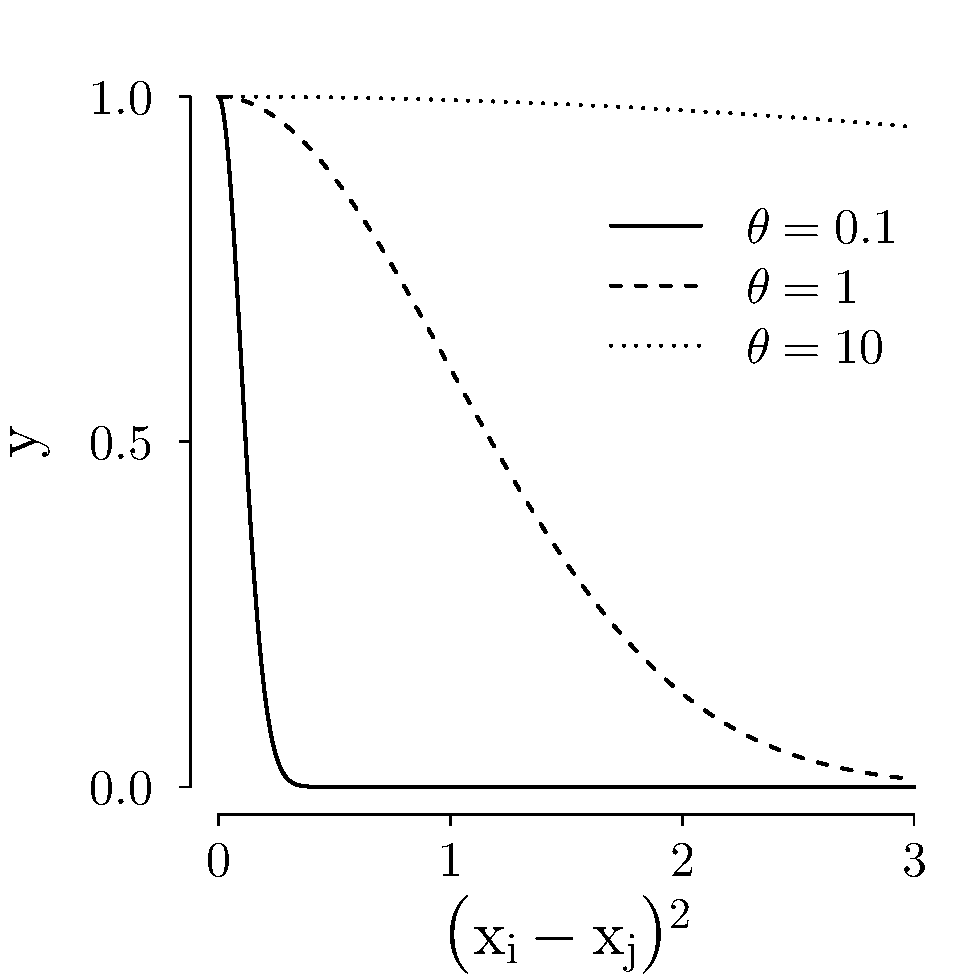
\includegraphics[scale=0.5]{../figures/chapter4/figures/plotCorrFunGauss.pdf}
	\caption[Gaussian correlation kernels with 3 different characteristic length scales]{Examples of Gaussian correlation kernels with 3 different characteristic length scales}
	\label{fig:plot_corrfun_gauss}
\end{figure}
As its name suggests, the characteristic length scale of a Gaussian kernel determines the scale or range of variation over the input domain.
To be precise, the notion how similar (or dissimilar) two input locations is defined relative to the characteristic length scale.
With a very short length scale, the output of random functions becomes uncorrelated easily except for the relatively very close (similar) inputs.
The realization of the process, therefore, will exhibit more erratic behavior in short length scale as it allows for more abrupt changes over shorter distance.
On the other hand, with a longer length scale, the output of random function tends to be highly correlated except for very different input values and thus the realization will exhibit more regular pattern.
Gaussian kernel, however, always produces smooth realization. That is, two input points that have a zero separation on the limit are both continuous and differentiable (see Fig.~\ref{fig:gaussian_kernel}).

Fig.~\ref{fig:plot_corrfun_gauss_realization} shows a comparison between realizations of a \gls[hyper=false]{gp} using Gaussian kernel for two different values of characteristic length scale.
The short length scale, illustrated on the left panel, allows for more sudden change in the output values while the long length scale on the right shows smoother (and rigid) pattern for the same input domain ($0.0 \leq x \leq 3.0$). 
Notice that the realizations, regardless of the length scale are smooth although as noted in, the shorter length scale produces more local maxima and minima in the realization.
The Gaussian kernel is parameterized by only a single \emph{hyper-parameter} $\theta$ that defines the characteristic length scale of the process (or simply \emph{the scale parameter}).
Fig.~\ref{fig:plot_corrfun_gauss} shows the correlation value as function of Euclidian distance, $(x_i - x_j)^2$, between input points according to the Gaussian kernel, 
for 3 different characteristic length scales.
Obviously, for smaller $\theta$ the correlation between two inputs drops more quickly over shorter distance, and vice versa.
%\begin{figure}[bth]
%	\centering
%	\includegraphics[scale=1.0]{../figures/chapter4/figures/plot_corrfun_gauss_realization.pdf}
%	\caption[Gaussian correlation kernels with 2 different characteristic length scales]{Examples of Gaussian correlation kernels with two different characteristic length scales}
%	\label{fig:plot_corrfun_gauss_realization}
%\end{figure}

\bigfigure[%pos=tbhp,
						%opt={},
						shortcaption={Stream tracing result.},
						label={fig:plot_corrfun_gauss}]
{../figures/chapter4/figures/plot_corrfun_gauss_realization.pdf}
{Damar}

\subsubsection{Power-Exponential Kernel}

\subsubsection{Mat\'ern Class Kernel}

\subsection{Multidimensional Construction}

In order to create a valid multidimensional correlation kernel function from a valid $1$-dimensional correlation function given above, 
a tensor product construction is used as follows,
\marginpar{tensor product}
\begin{equation}
	R(\mathbf{x}_i, \mathbf{x}_j) = \prod_{d = 1}^{D} r_d \left(x_i^{(d)}, x_j^{(d)}\right)
\label{eq:tensor_product}
\end{equation}
where $r_d$ is a $1$-dimensional correlation kernel function for the $d$-th input dimension;
while $x_i^{(d)}$ and $x_j^{(d)}$ are a pair of values in the $d$-th input dimension.

Although it is possible to mix different types of correlation function or use different kind of multidimensional construction (see for example \cite{Higdon2002}),
the tensor product with the same correlation function for each input dimension is the most well-established 
and, by far, the most popular approach in the applied metamodeling literature to date \cite{Roustant2012,Sacks1989,Sacks1989a,Santner2003,Currin1991,Marrel2008,Bachoc2014,Kennedy2006,Jones2009}.

Fig.~\ref{fig:random_surfaces} shows two examples of realizations of random surface drawn from a multidimensional \gls[hyper=false]{gp} with the same process variance ($\sigma^2 = 10.0$) but with two different correlation kernels.
On the left is an example of a realization drawn from the \gls[hyper=false]{gp} using Gaussian correlation kernel function with relatively the characteristic length scale in $y$-direction is four times the scale in $x$-direction.
On the right is an example of a realization drawn from the \gls[hyper=false]{gp} using Mat\'ern correlation kernel function.
For this case, the shape parameter is three times larger in the $x$-direction than in the $y$-direction.
As such, for both cases, the surface appears less smooth in one of the direction.
\bigdoublefigure[pos=tbhp,
                 mainlabel={fig:random_surfaces},
								 mainshortcaption={Random surface realizations},
                 maincaption={Two random surfaces drawn from two different multidimensional \gls[hyper=false]{gp} with the same process variance of $\sigma^2 = 9.0$. Differences in the scale (for Gaussian) and shape (for Mat\'ern) parameters for the inputs yield smoother path in one direction. The color scheme is the same for both plots with the range of $\pm \, 3 \times \sigma$.},
                 leftopt={width=0.475\textwidth},
                 leftlabel={fig:random_surface_gaussian},
                 leftcaption={Gaussian, $\theta_x = 0.5, \theta_y = 2.0$},
                 rightopt={width=0.475\textwidth},
                 rightlabel={fig:random_surface_matern},
                 rightcaption={Mat\'ern, $\theta_x = 1.5, \theta_y = 0.5$},
                 ]
{../figures/chapter4/figures/plotRandomSurface_1}
{../figures/chapter4/figures/plotRandomSurface_2}

\subsection{Process Variance}

For stationary \gls[hyper=false]{gp}, the shape of sample path is determined solely by the form of the correlation.
The role of process variance according to Eq.~(\ref{eq:cov_function}) is to determine the scale of magnitude of output variation. 
Fig.~\ref{fig:plot_process_variance} gives an illustration of realizations drawn from a set of \glspl[hyper=false]{gp} with the same kernel correlation function (i.e., Gaussian kernel with $\theta = 1.0$), 
but with different values of process variance.
As it can be seen, the visible features of the realizations remain the very similar to each other.
What has changed, however, is the scale of the variation in the output space.  
\bigtriplefigure[pos=tbhp,
								 mainlabel={fig:plot_process_variance},
			           maincaption={Realizations of \gls[hyper=false]{gp} with Gaussian correlation kernel for $3$ different values of process variance. The plotting range of the $y$-axis for each panel are set to $\pm \, 3 \times \sigma$.},
			           mainshortcaption={Bundle collision strategies.},%
			           leftopt={width=0.30\textwidth},
			           leftlabel={fig:plot_process_variance_1},
			           leftcaption={},
			           midopt={width=0.30\textwidth},
			           midlabel={fig:plot_process_variance_2},
			           midcaption={},
			           rightopt={width=0.30\textwidth},
			           rightlabel={fig:plot_process_variance_3},
			           rightcaption={},
			           spacing={},
			           spacingtwo={}]
{../figures/chapter4/figures/plotProcessVariance_1}
{../figures/chapter4/figures/plotProcessVariance_2}
{../figures/chapter4/figures/plotProcessVariance_3}

\subsection{Mean Function}